\documentclass[aps,12pt,prd,nofootinbib,bibnotes, amsmath,amssymb,showpacs,superscriptaddress,floatfix]{revtex4-2}
\bibliographystyle{apsrev}
\usepackage[utf8]{inputenc}
\usepackage{epsf,epsfig,graphics}
\usepackage{graphicx,amsmath,mathrsfs,amssymb, amsthm,nccbbb,cancel,xcolor,wrapfig,siunitx,longtable,tabularx,CJKutf8,subfigure,float,xspace,physics,esvect,braket,enumitem,url,makeidx}
\usepackage{verbatim,color,ulem}
\usepackage{bm}
\usepackage[mathscr]{eucal}
\usepackage{hyperref}
\usepackage[toc,page]{appendix}
\usepackage[hang, flushmargin]{footmisc}
\usepackage{footnotebackref}

%%%%%%%%%%%%%%%%%%%%%%%%%%%%%%%%%%%%%%%%%%%
\begin{document}
\title{Computational Astrophysics HW6}
\author{Yi-Hsiang Kuo, 110022506}
\date{Dec. 22, 2022}
\maketitle
%\tableofcontents
%%%%%%%%%%%%%%%%%%%%%%%%%%%%%%%%%%%%%%%%%%%
\section{Exercise 1}
By implementing the definition of  {\bf{face-averaged magnetic fields}} and the {\bf{line-averaged EMFs}} in $n+1$ step, we'll find that the $\epsilon$ part will all be cancelled out. Hence the divergence free constraint can be conserved. 
\begin{figure}[H] 
\centering 
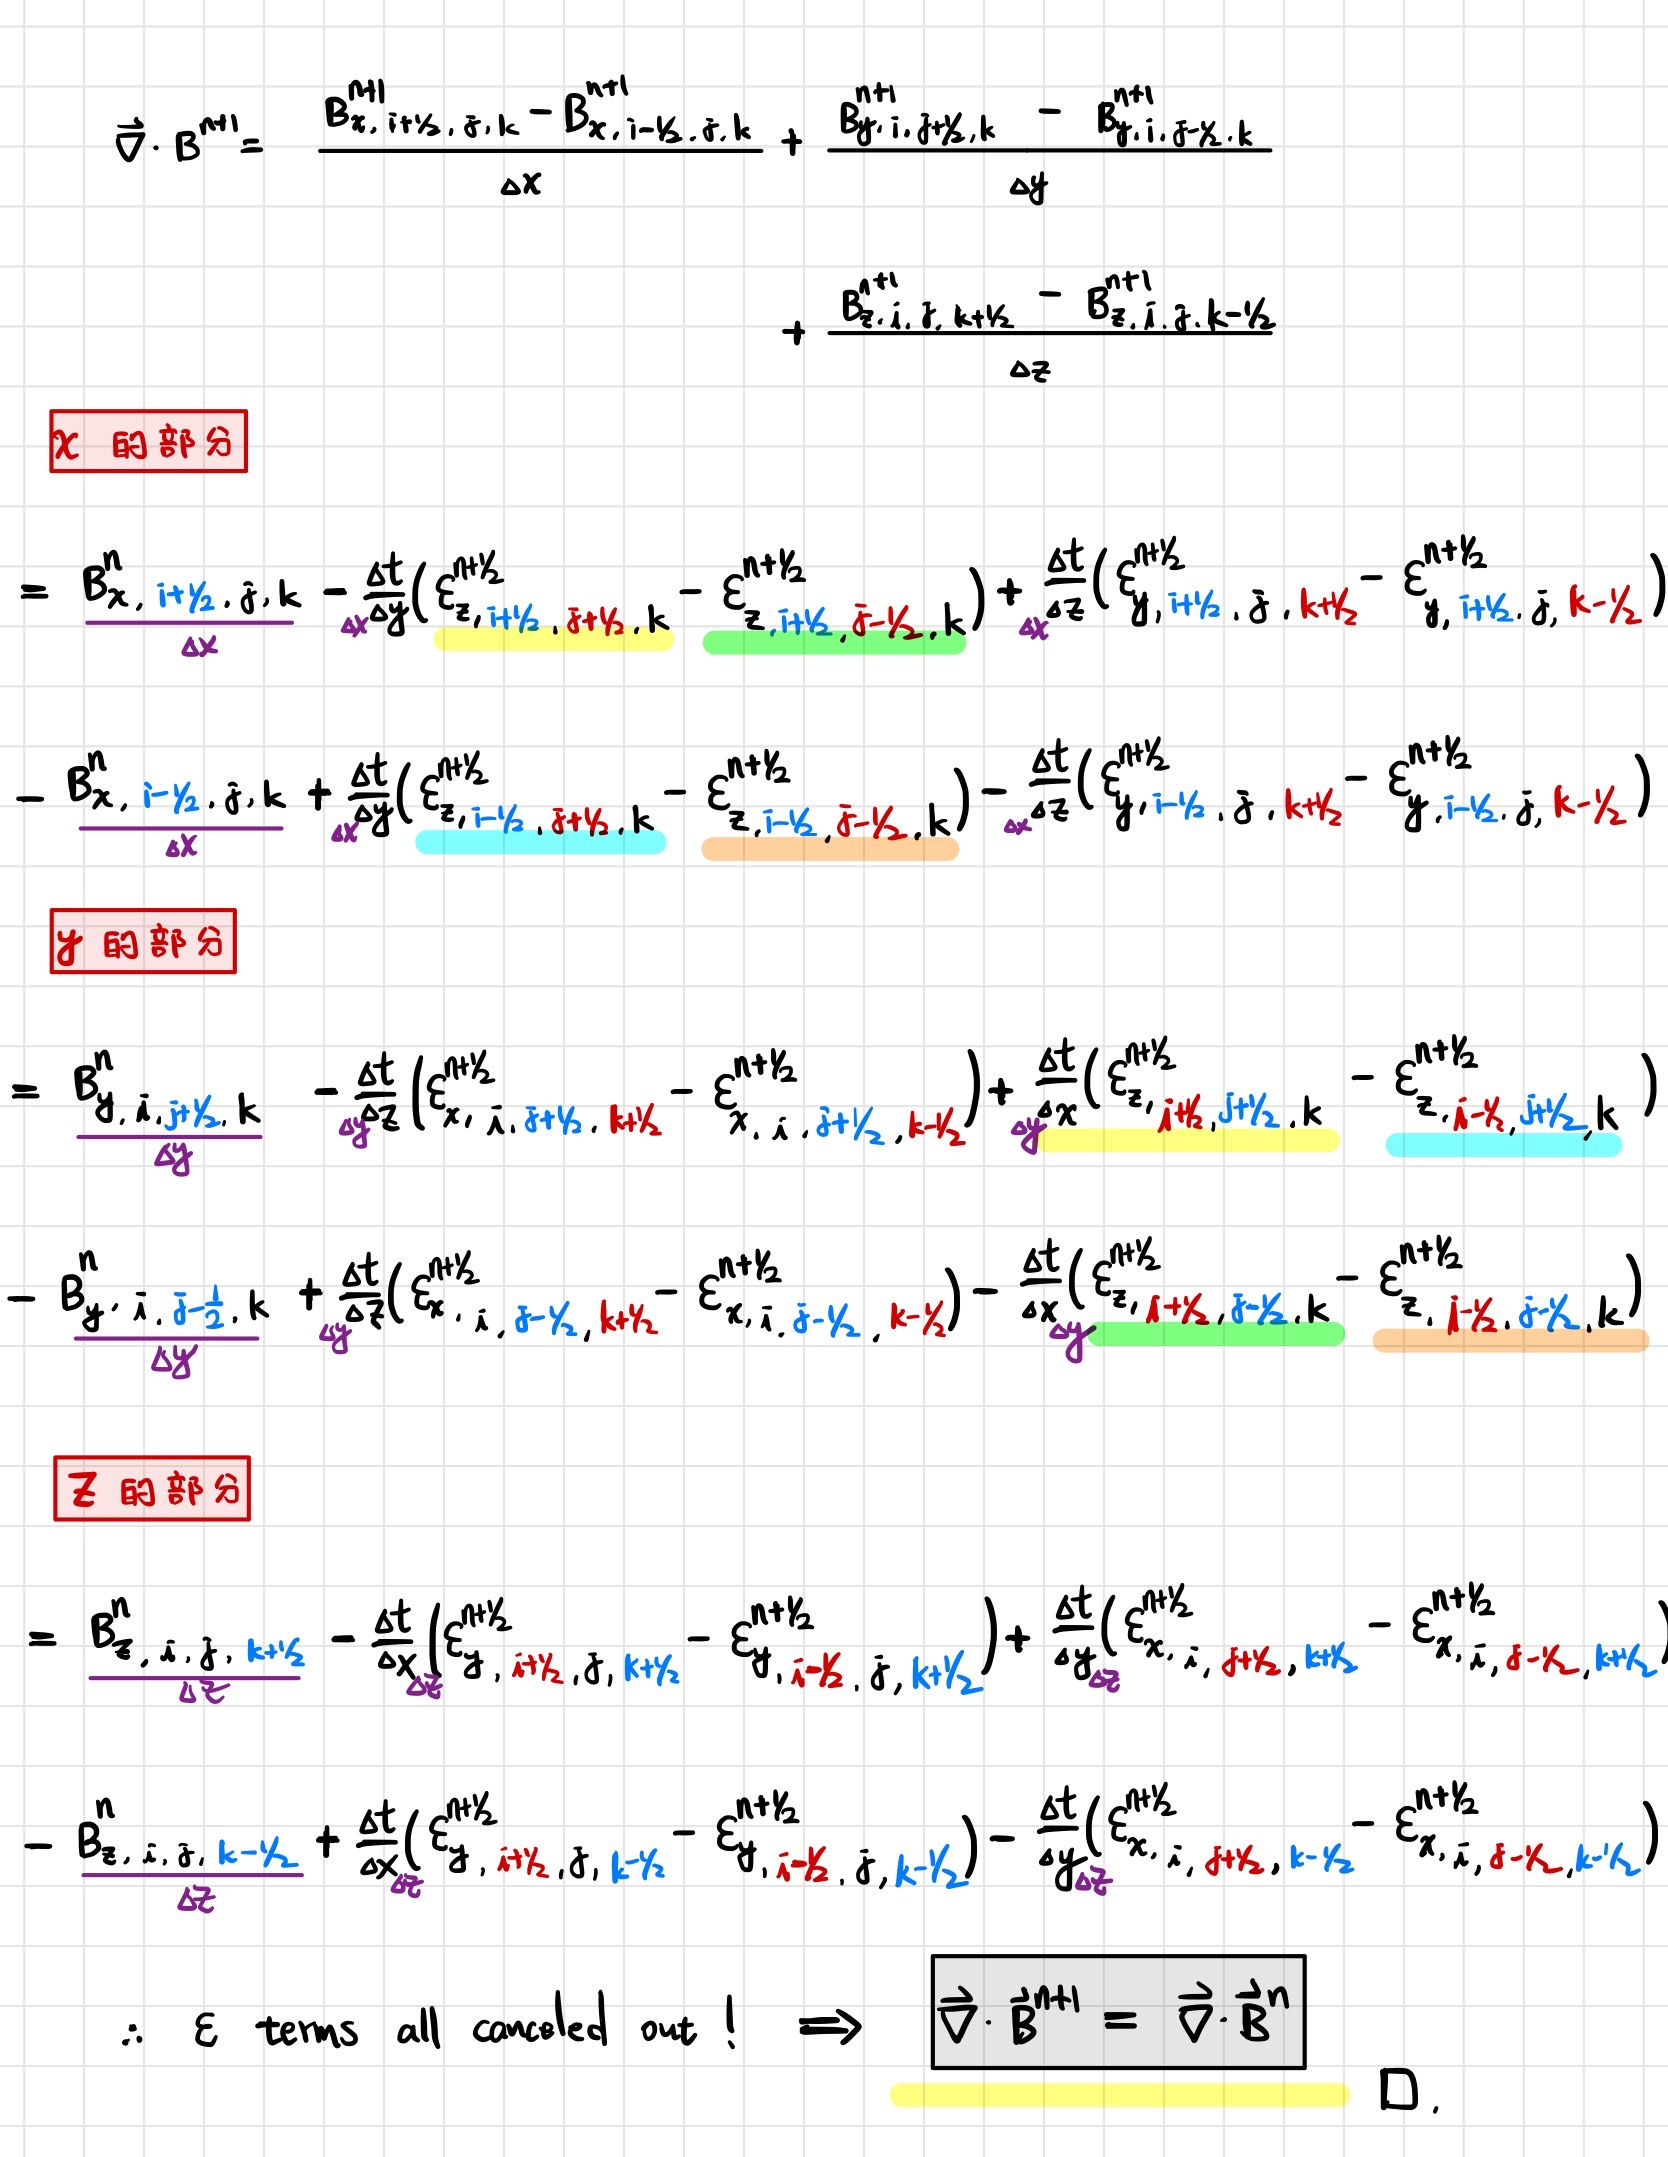
\includegraphics[width=0.7\textwidth]{EX1} 
\caption{Calculation}  
\end{figure}
    
\section{Exercise 2}
(1)Implement the SOR method, and rum the code with $\omega = 1.2$, the result shows that SOR method converge faster than the Jacobi and GS methods
\begin{figure}[H]
\centering  
\subfigure[Jacobi method]{
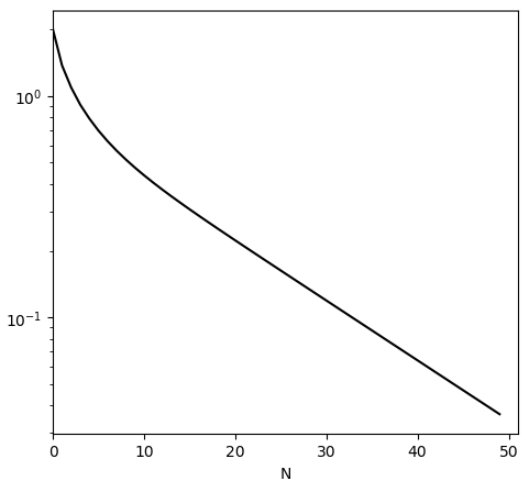
\includegraphics[width=0.45\textwidth]{EX2-1}}
\subfigure[GS method]{
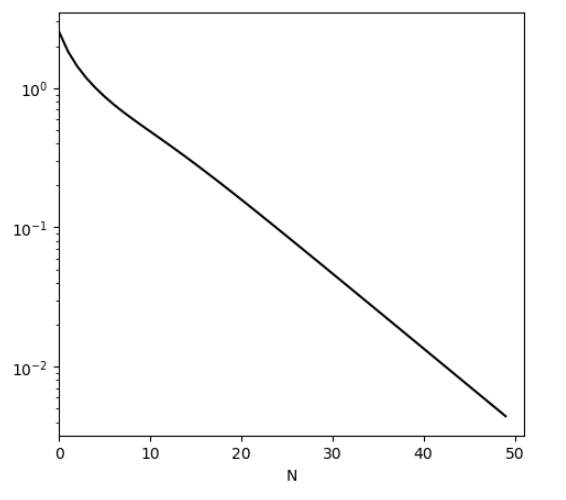
\includegraphics[width=0.45\textwidth]{EX2-2}}
\subfigure[SOR method]{
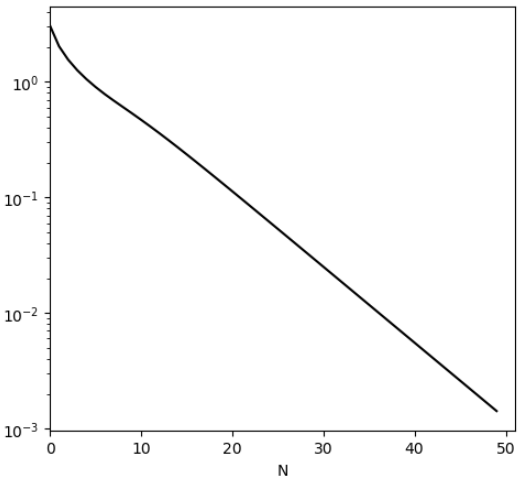
\includegraphics[width=0.45\textwidth]{EX2-3}}
\caption{Methods comparison}
\end{figure}

(2)
\section{Exercise 3}

(1) The paper I choose (link is put below) is {\bf{Fundamental differences between SPH and grid methods}}, they found that by using these two method modelling fundamental process across many areas of astrophysics (e.g. {\bf{Kelvin-Helmholtz instability}}, {\bf{Rayleigh-Taylor instability}})

The main set-up is a blob test: A spherical cloud of gas is placed in a wind tunnel, so as to investigate how different simulation codes affect the typical astrophysical processes. \\
   
(2) The numerical simulation is done under the following condition: \\
{\bf{Neglect physical viscosity}} and {\bf{radiative process}}, assume the gas evolution is strictly {\bf{adiabatic}}. \\  

 The initial condition for SPH code is a specular particle set-up, for grid-based simulations, the initial condition are obtained by smoothing the gas quantities on to each cell centre using the same spline kernel as in the SPH codes using 32 nearest neighbours.\\

There are several simulation codes, however, they all give similar results for grid-based and SPH codes.\\
 
(3) The main result is as the figure in Teacher's lecture, the gas density seems pretty different for 2 methods. The grid-based simulation clearly shows the completely fragmentation after a certain timem unlike the SPH simulations. 
\begin{figure}[H] 
\centering 
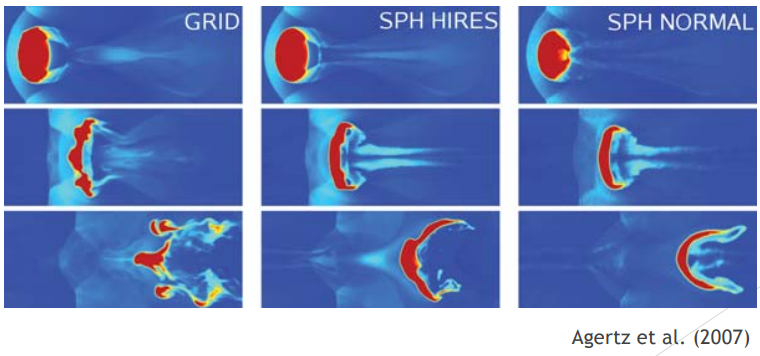
\includegraphics[width=0.7\textwidth]{EX3} 
\caption{A screen shot from lecture note 14}  
\end{figure}

(4) The probable reason contributes to the difference is that for SPH method, introduces a spurious{\bf{shear force}} which causes the interaction are severely damped.

\section{Code link}
\href{https://github.com/kuo1235/Computational-Astrophysics-2022/blob/main/astr660/Homework/HW6/EX2/laplace_template_L13\%20(1).ipynb}{\textcolor{blue}{\bf{Exercise2}}} 

\href{https://academic.oup.com/mnras/article/380/3/963/952655}{\textcolor{blue}{\bf{Exercise3-Reference}}}


\bibliography{Ref}
\end{document}







